\section{Einführung}

Dieses Projekt widmet sich der Umsetzung eines Drumcomputers, einem elektronischen Musikinstrument, das die Erzeugung und Steuerung perkussiver Klänge ermöglicht. Ein Drumcomputer bietet die Möglichkeit, individuelle Rhythmen zu generieren und abzuspielen, was beispielsweise als Begleitung für Solokünstler von großem Nutzen ist. Der von uns entwickelte Drumcomputer kombiniert analoge Klangerzeugung mit moderner Digitaltechnologie, die eine Steuerung der Klänge über einen Computer ermöglicht. Das Projekt beinhaltet Themen der Digitalen Datenkommunikation, und der Analogen Schaltungstechnik.

Die Grundlage für die Klangerzeugung dieses Projekts beruht auf den Anfängen der elektronischen Musik in den 1970er und 80er Jahren. Es werden insgesamt acht verschiedene Klänge erzeugt, die mithilfe analoger Schwingkreise realisiert werden: Bassdrum (Große Trommel), zwei Snaredrums (Schnarrtrommeln), Cymbal (Becken), Clave (Klanghölzer), Maracas (Rumba-Rasseln) und zwei Congas (lateinamerikanische Trommeln). Diese Klänge können entweder einzeln über einen Taster abgespielt oder vom Mikrocontroller gesteuert werden. Der Mikrocontroller empfängt Signale über die MIDI-Schnittstelle und nutzt diese zur Steuerung der Klänge. MIDI ist der \enquote{Industriestandard für den Austausch musikalischer Steuerinformationen zwischen elektronischen Instrumenten} \cite{wiki_midi} und ermöglicht die Integration der Klänge in die Struktur anderer elektronischer Klangsysteme.

Das Gerät ist im Eurorack-Format konzipiert, um eine nahtlose Integration zu gewährleisten. Eurorack ist ein standardisiertes Format für den Bau von Modulen für modulare Synthesizer. Im folgenden Abschnitt wird eine kurze Einführung in modulare Synthesizer gegeben, um das Gesamtprojekt besser zu verstehen und den Kontext zu erläutern.

\subsection{Einführung modularer Synthesizer}

\begin{figure}[H]
    \centering
    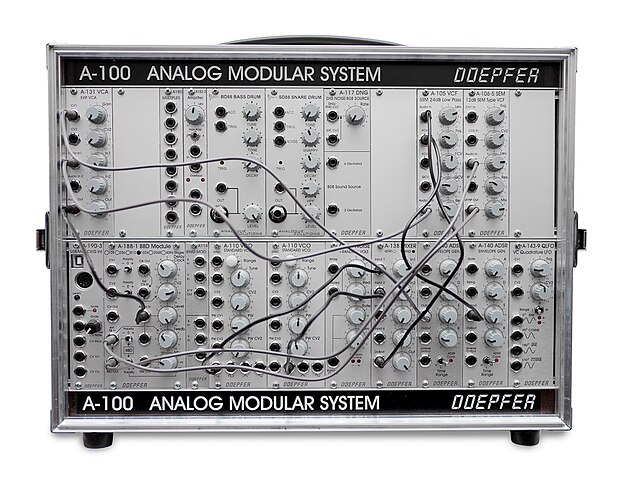
\includegraphics[width=0.8\textwidth]{Images/Modularer Synthesizer.jpg}
    \caption[Modularer Synthesizer]{Modularer Synthesizer \cite{wiki_eurorack}}
    \label{fig:Modularer Synthesizer}
\end{figure}

Modulare Synthesizer repräsentieren eine Kategorie von elektronischen Musikinstrumenten, die aufgrund ihrer modularen Struktur eine umfassende Kontrolle über die Klanggenerierung ermöglichen. Der Klang, der schließlich über einen Lautsprecher wiedergegeben wird, setzt sich aus vielfältigen Komponenten zusammen, die in einzelne Module unterteilt sind. 


Die Modularität dieser Synthesizer ermöglicht den Austausch von Modulen sowie die Integration neuer Module. Jedes Modul verfügt über individuelle Parameter, die auch von anderen Modulen beeinflusst werden können. Ein konkretes Beispiel hierfür ist der Voltage-Controlled-Filter (kurz VCF), der durch externe Signale gesteuert werden kann.

Die Verbindung zwischen den einzelnen Modulen erfolgt mithilfe von Kabeln. Jedes Modul verfügt über Ein- und Ausgänge, die den modularen Aufbau ermöglichen und eine flexible Signalverarbeitung ermöglichen.

Das in diesem Projekt entwickelte modulare Drumcomputer-System wurde konzipiert, um die unabhängige Bearbeitung der verschiedenen Klangkomponenten zu ermöglichen. Dadurch können die Klänge separat voneinander verändert und angepasst werden.

Wie bereits in der Einleitung erwähnt, wurde dieses Projekt gemäß dem Eurorack-Standard entwickelt. Das Eurorack stellt eine Stromversorgung für alle Module bereit, wobei die Versorgungsspannungen für die Module bei +12 V, -12 V und +5 V liegen. Der Standard besagt, dass für Trigger Signale 5 V vorgesehen sind. Audio Signale besitzen eine 10 Volt Peak-to-Peak Spannung, für einen besseren Rauschabstand. Zusätzlich sind Pins für Gate- und Steuerspannung (Control Voltage) vorhanden, jedoch werden diese in diesem Projekt nicht verwendet.

%Signale erklären: Gate, Trigger, Control Voltage, Audio
% kurz erläutern, dass auch die bauform der module standardisiert ist